\documentclass[compress,pdftex%draft
]{beamer}
\usepackage[overlay,absolute,
%showboxes
]{textpos}

\include{highlight.css}

\usepackage{listings}
\usepackage{etex}
%%%%%%%%%%%
% fonts for listing
%%%%%%%%%%%
% \defaultfontfeatures{Scale=MatchLowercase}
% \setmainfont[Mapping=tex-text]{Georgia}
% \setsansfont[Mapping=tex-text]{Arial}
% \setmonofont{Courier New}
%%%%%%%%%%%
\usepackage[usenames,dvipsnames]{pstricks}
\usepackage{epsfig}
\usepackage{pst-grad} % For gradients
\usepackage{pst-plot} % For axes
\usepackage{epstopdf}

\usepackage{proof}
\usepackage{calrsfs}
%\usepackage{ICALPbeamerthemeshadow}
\usepackage{amsmath,stmaryrd,amssymb,latexsym,rotating}
\usepackage[latin1]{inputenc}
\usepackage[english]{babel}
\usepackage{alltt}
\usepackage{graphics}
%\usepackage[cspex]{mathbbol}
\usepackage[all]{xy}

%%%%%%%%%%%%%%% from icalp
\newcommand{\altt}{~~|~~}
\newcommand{\para}{~~|~~}
\newcommand{\zero}{\mathbf{0}}
\newcommand{\one}{\mathbf{1}}
\newcommand{\accept}[1]{\pmb{\lbag} #1 \pmb{\rbag}}
\newcommand{\cqlp}{$\mathbb{C}${\rm QL}{}$_P$}
\newcommand{\cqlx}{$\mathbb{C}${\rm QL}{}$_X$}
\newcommand{\cduce}{$\mathbb{C}${\rm Duce}}
\newcommand{\cql}{$\mathbb{C}${\rm QL}}
\newcommand{\duce}{$\mathbb{C}${\rm Duce}}
\newcommand{\C}[1]{{\fontfamily{cmtt}\fontencoding{T1}\fontseries{c}\fontshape{sl} %
\fontsize{10}{11pt}\selectfont \textrm{#1}}}
\newcommand{\msf}[1]{\textsf{#1}}
% Les motifs
\newcommand{\pator}[2]{#1 \msf{|} #2}
\newcommand{\patand}[2]{#1 \msf{\wedge} #2}
%\newcommand{\patleft}[1]{\msf{(}#1\msf{,\_)}}
%\newcommand{\patright}[1]{\msf{(\_,}#1\msf{)}}
\newcommand{\patcst}[2]{\msf{(}#1\msf{:=}#2\msf{)}}
\newcommand{\patpair}[2]{\msf{(}#1\msf{,}#2\msf{)}}
%\newcommand{\patpair}[2]{\blpar #1 \boldsymbol{,} #2 \brpar}
\newcommand{\Is}{\colon\!\!\colon \!\!\!\!= }
\newcommand{\expr}{{e}}
\newcommand{\pat}{{\tt p}}
\newcommand{\const}{{c}}
\newcommand{\op}{{o}}
\newcommand{\ops}{{\mathbb O}}
\newcommand{\valeurs}{{\cal V}}
\newcommand{\blpar}{\boldsymbol{(}}
\newcommand{\brpar}{\boldsymbol{)}}
\newcommand{\match}[5]{\mathtt{match~} #1 \mathtt{~with~} #2 \myarrow #3 \mybar
  #4 \myarrow #5}
\newcommand{\typecase}[5]{\mathtt{typecase~} #1 \mathtt{~with~} (#2 :
  #3) \myarrow #4 \mybar (#2 : \synneg #3) \myarrow #5}
\newcommand{\typec}[5]{\texttt{(} #3=#1\pmb{\in}#2\texttt{)}\pmb{?}#4\texttt{{:}}#5}
\newcommand{\genabstraction}[3]{\abstr{f}{#1}{#2}{#3}}
\newcommand{\abstr}[4]{\boldsymbol{\mu} #1^{\blpar #2 \brpar}\blpar #3 \brpar \boldsymbol{.}#4}
\newcommand{\stdmatch}{\match{\expr}{p_1}{\expr_1}{p_2}{\expr_2}}

% \newcommand{\exprpair}[2]{\blpar #1 \boldsymbol{,} #2 \brpar}

\newcommand{\exprop}[2]{#1 \blpar #2 \brpar}
\newcommand{\slide}[2]{\begin{frame}\frametitle{#1}#2\end{frame}}
\newcommand{\syntimes}{{\pmb{\times}}}
\newcommand{\synprod}{{\pmb{\times}}}
\newcommand{\synarrow}{{\pmb{\rightarrow}}}
\newcommand{\synneg}{{\pmb{\neg}}}
\newcommand{\synvee}{{\pmb{\vee}}}
\newcommand{\synwedge}{{\pmb{\wedge}}}
\newcommand{\syndiff}{{\pmb{\backslash}}}
\newcommand{\syncap}{\operatornamewithlimits{\pmb{\bigwedge}}}
\newcommand{\syncup}{\operatornamewithlimits{\pmb{\bigvee}}}
\newcommand{\reff}{\mathtt{ref}\,}
\newcommand{\lazy}{\mathtt{lazy}\,}
\newcommand{\synchan}[1]{\textit{ch}(#1)}
\newcommand{\synchanout}[1]{\textit{ch}^-(#1)}
\newcommand{\synchanin}[1]{\textit{ch}^+(#1)}

\newcommand{\sem}[1]{{\llbracket {#1} \rrbracket}}
\renewcommand{\subset}{\subseteq}
\newcommand{\values}{\mathcal{V}}
\newcommand{\domaine}{\mathcal{D}}
\newcommand{\stdmod}{\mathcal{U}}
\renewcommand{\P}{\mathcal{P}}
\newcommand{\Pf}{\mathcal{P}_{\!f}}
\newcommand{\exten}{\mathbb{E}}


\newcommand{\Ll}[1]{\small$\mathcal{P}\llbracket$ #1 $\rrbracket$}
\newcommand{\Hl}[1]{$\mathcal{H}\llbracket$#1 $\rrbracket$}
\newcommand{\F}[2]{\small$\mathcal{F}\llbracket$ #1 $\rrbracket_{#2}$}
\newcommand{\Sl}[1]{$\mathcal{S}\llbracket$ #1 $\rrbracket$}
\newcommand{\W}[1]{$\mathcal{W}\llbracket$ #1 $\rrbracket$}
% nom de l algo de reecriture
\newcommand{\R}[1]{$\mathcal{R}$(#1)}
\newcommand{\s}{\hspace*{2mm}}
%%%%%%%%%% end from icalp

\newcommand{\ignore}[1]{}
\newif{\ifSHORTER}
\SHORTERtrue
\SHORTERfalse
\usepackage{pgfarrows}
% Try the class options [notes], [notesonly], [trans], [handout],
% [red], [compress], [draft] and see what happens!

% Copyright 2003 by Till Tantau <tantau@users.sourceforge.net>.
%
% This program can be redistributed and/or modified under the terms
% of the LaTeX Project Public License Distributed from CTAN
% archives in directory macros/latex/base/lppl.txt.

% For a green structure color use:
\colorlet{structure}{green!50!black}
\definecolor{ocre}{rgb}{.41,.34,0}
\definecolor{lightgreen}{rgb}{0.79,0.86,.79}
\definecolor{lesslightgreen}{rgb}{0.39,.9,.39}
\definecolor{mydarkgreen}{rgb}{0.10,0.43,0}
\usetheme{Warsaw}
\setbeamercovered{dynamic}


\newcommand<>{\mypmb}[1]{\only#2{\pmb}{#1}}
\newcommand{\myalert}[2]{{\only<#1>{\color{red}}{#2}}}

\beamerboxesdeclarecolorscheme{point}{blue}{blue!15!averagebackgroundcolor}
\beamerboxesdeclarecolorscheme{good}{green}{green!15!averagebackgroundcolor}
\beamerboxesdeclarecolorscheme{bad}{red}{red!15!averagebackgroundcolor}

\definecolor{darkgreen}{rgb}{0,0.65,0.08}
\definecolor{darkblue}{rgb}{0,0.08,0.55}

\newcommand{\beamerbullet}[1]{
  \begin{pgfpicture}{-1ex}{-0.55ex}{1ex}{1ex}
    \usebeamercolor[fg]{subitem projected}
    \begin{pgfmagnify}{1.4}{1.4}
      \pgfbox[center,center]{\normalsize\pgfuseshading{bigsphere}}
    \end{pgfmagnify}
    \pgfbox[center,center]{%
      \usebeamerfont*{subitem projected}%
      #1}
  \end{pgfpicture}%
}

\newcommand{\beamerbigbullet}[1]{
  \begin{pgfpicture}{-1ex}{-0.65ex}{1ex}{1ex}
    \usebeamercolor[fg]{item projected}
    \begin{pgfmagnify}{1.75}{1.75}
      \pgfbox[center,center]{\normalsize\pgfuseshading{bigsphere}}
    \end{pgfmagnify}
    \pgfputat{\pgfpoint{0pt}{0.5pt}}
    {%
      \pgfbox[center,center]{%
        \usebeamerfont*{item projected}%
        #1}}
  \end{pgfpicture}%
}

\newcommand{\beamerhugebullet}[1]{\leavevmode\leftskip=2.75ex%
  \llap{%
    \normalsize%
    \begin{pgfpicture}{-1ex}{-0.7ex}{1ex}{1ex}
    \usebeamercolor[fg]{item projected}
      \pgfbox[center,center]{\normalsize\pgfuseshading{tocsphere}}
      \pgfbox[center,center]{%
        \usebeamerfont*{section number projected}%
        \usebeamercolor{section number projected}%
        \color{fg!90!bg}%
        #1}
    \end{pgfpicture}%
    \kern1.25ex}%
%  #1\par
}

\newcommand{\pointbox}[2]
{\begin{beamerboxesrounded}[scheme=point,shadow=true]{#1}{#2}
 \end{beamerboxesrounded}}

\newcommand{\goodbox}[2]
{\begin{beamerboxesrounded}[scheme=good,shadow=true]{#1}{#2}
 \end{beamerboxesrounded}}
\newcommand{\badbox}[2]
{\begin{beamerboxesrounded}[scheme=bad,shadow=true]{#1}{#2}
 \end{beamerboxesrounded}}

\hypersetup{%
  pdftitle={Autour d'XML, hors des standards : types, langages ...},
  pdfauthor={V\'eronique Benzaken},
  pdfsubject={Theoretical Computer Science},
  pdfkeywords={XML,query,programming languages}}
\usepackage{colortbl}


%
%
%  END OF BEAMER SPECIFIC OPTIONS
%
%



%\newcommand{\syntimes}{{\pmb{\times}}}
%\newcommand{\synprod}{{\pmb{\times}}}
%\newcommand{\synarrow}{{\pmb{\rightarrow}}}
%\newcommand{\synneg}{{\pmb{\neg}}}
%\newcommand{\synvee}{{\pmb{\vee}}}
%\newcommand{\synwedge}{{\pmb{\wedge}}}
%\newcommand{\syndiff}{{\pmb{\backslash}}}
%\newcommand{\syncap}{\operatornamewithlimits{\pmb{\bigwedge}}}
%\newcommand{\syncup}{\operatornamewithlimits{\pmb{\bigvee}}}

%\newcommand{\altt}{{\color{black}~~|~~}}
%\newcommand{\zero}{\mathbb{0}}
%\newcommand{\one}{\mathbb{1}}
%\newcommand{\accept}[1]{\pmb{\lbag} #1 \pmb{\rbag}}
%\newcommand{\cqlp}{$\mathbb{C}${\rm QL}{}$_P$}
%\newcommand{\cqlx}{$\mathbb{C}${\rm QL}{}$_X$}
%\newcommand{\cduce}{$\mathbb{C}${\rm Duce}}
%\newcommand{\cql}{$\mathbb{C}${\rm QL}}
%\newcommand{\duce}{$\mathbb{C}${\rm Duce}}
%\newcommand{\C}[1]{{\fontfamily{cmtt}\fontencoding{T1}\fontseries{c}\fontshape{sl} %
%\fontsize{10}{11pt}\selectfont \textrm{#1}}}
%\newcommand{\msf}[1]{\textsf{#1}}
% Les motifs
%\newcommand{\pator}[2]{#1 \msf{|} #2}
%\newcommand{\patand}[2]{#1 \msf{\wedge} #2}
%\newcommand{\patleft}[1]{\msf{(}#1\msf{,\_)}}
%\newcommand{\patright}[1]{\msf{(\_,}#1\msf{)}}
%\newcommand{\patcst}[2]{\msf{(}#1\msf{:=}#2\msf{)}}
%\newcommand{\patpair}[2]{\msf{(}#1\msf{,}#2\msf{)}}
%\newcommand{\patpair}[2]{\blpar #1 \boldsymbol{,} #2 \brpar}


%\newcommand{\Ll}[1]{\small$\mathcal{P}\llbracket$ #1 $\rrbracket$}
%\newcommand{\Hl}[1]{$\mathcal{H}\llbracket$#1 $\rrbracket$}
%\newcommand{\F}[2]{\small$\mathcal{F}\llbracket$ #1 $\rrbracket_{#2}$}
%\newcommand{\Sl}[1]{$\mathcal{S}\llbracket$ #1 $\rrbracket$}
%\newcommand{\W}[1]{$\mathcal{W}\llbracket$ #1 $\rrbracket$}
%% nom de l algo de reecriture
%\newcommand{\R}[1]{$\mathcal{R}$(#1)}
%\newcommand{\s}{\hspace*{2mm}}

%%%%%%%%%%%%%%%%%%%%%%%%%%%%
% define new command
\newcommand{\bdm}
{
\begin{displaymath}
\begin{array}{rcl}
}
\newcommand{\edm}
{
\end{array}
\end{displaymath}
}
\newcommand{\bda}[1]
{
\begin{displaymath}
\begin{array}{#1}
}
\newcommand{\eda}
{
\end{array}
\end{displaymath}
}
\newcommand{\UB}{U(\mathcal{B})}
\newcommand{\Ur}{U(r)}
\newcommand{\lvec}[1]{\stackrel{\leftarrow}{#1}}
\newcommand{\rvec}[1]{\stackrel{\rightarrow}{#1}}
%%%%%%%%%%%%%%%%%%%%%%%%%%%%

\title[Automated constraint verification for databases\hspace{16mm} \insertframenumber/\inserttotalframenumber]{\bf Automated constraint verification for databases}
\author[Shuai Yuan]{%
  Shuai Yuan \\
 advised by V\'eronique Benzaken, Evelyne Contejean \\
 and Mingli Song}
\institute[LRI - CNRS,  U. Paris Sud XI ]{
  Universit\'e de Paris Sud XI \\
  LRI, CNRS}
\institute[zjucs]{
College of Computer Science and Technology, \\
Zhejiang University  
}

\date[GT Proval]{}

%\pgfdeclareimage[width=1cm]{logoENS}{logoENS}
%\logo{\hbox{\pgfuseimage{logoENS}}}



%\usepackage{pst-node,pst-tree}
\usepackage{graphicx}
%\usepackage{color}
%\usepackage{epsfig}
%\usepackage{rotating}

% support Chinese fonts
% \usepackage{cctbase}

\begin{document}

\frame{\titlepage}
\frame{\frametitle{Outline}
\begin{itemize}
\item Background
\item Context
\item Proposed solutions
\item Database integrity constraints
\item SQL data modification operations
\item Why3
\item Translation overiew
\item Problem and solutions
\item Experiments
% \item Example
% \item Demo
\item Conclusion and perspectives
\end{itemize}
}

\section[1.\ Background --\!\!]{Background}
\begin{frame}
\frametitle{Background}

\begin{itemize}
  \item<1> {Integrity constraints are important to express the semantics of databases.}
	\begin{itemize}
	  \item prevent the execution of operations or transactions which will cause violation of constraints
	  \item semantics query optimization
	\end{itemize}
  \item<2> {No real DBMS (database management system) have fully support the management of integrity constraints. \\
	i.e. assertions which are part of the SQL standard}
  \item<3-> {The alternative solution widely adopted by main-stream DBMS -- triggers:}
	\only<3>{
	  \begin{itemize}
		\item \color{blue}{event}
		\item \color{blue}{condition}
		\item \color{blue}{action}
	  \end{itemize}
	}
	\only<4>{
	\begin{itemize}
	  \item Integrity is spread out among several triggers and therefore the global vision of the semantics is lost.
	  \item The behavior of triggers is complex (cascading, conflict, \textit{etc.}).
	\end{itemize}
  }
\end{itemize}

\end{frame}

\section[2.\ Context --\!\!]{Context}

\frame{\frametitle{Context}
We have:
% \pause
% \begin{itemize}[<+->]
\begin{itemize}
     \item {\color{blue}{database}} $\mathcal{B}$.
     \item<2-> {\color{blue}{database integrity constraint}} $C$.
	   \only<4>
	   {
		 \begin{enumerate}
		   \item domain constraint
		   \item column constraint
		   \item table constraint
		   \item assertion
		 \end{enumerate}
	   }
			 % , which is expressed by SQL assertion.
     \item<3-> {\color{blue}{data modification operation}} $U$.
	   % , which will change the state of $\mathcal{B}$. \\
	   \only<4>
	   {
		 \begin{enumerate}
		   \item INSERT
		   \item DELETE
		   \item UPDATE
		 \end{enumerate}
	   }
	   % three kinds of updates in SQL: {\color{red}{INSERT, DELETE, UPDATE}}.
\end{itemize}
% \pause
% \begin{itemize}
%      \item<2-> {\color{blue}{SQL Assertion}}: the general form of integrity constraint of database.
%
%      \item<3-> {\color{blue}{SQL updates}}: functions that will change the state of database. There are three kinds of update functions in SQL: {\color{red}{INSERT, DELETE, UPDATE}}
%
% \end{itemize}

\only<4>{
%
\begin{center}
  We focus on {\color{darkgreen}{relational databases}} and {\color{darkgreen}{SQL}}.
\end{center}
}

\bigskip
\pause
\only<5>{
Before $U$ is executed, $\mathcal{B} \models C$ \\
What we want to prove:
After $U$ is executed, $\UB \models C$. \\
\begin{center}
% $U$ preserves constraint $C$.
$U$ preserves $C$,
or $U$ is safe with respect to $C$, \\
if for any database $\mathcal{B}$:
\[
  \mathcal{B} \models C \Rightarrow \UB \models C
\]
\end{center}
% Proof target: \\
% if the database satisfies the assertion before an update, \\
% after executing the update, the constraints will still be presearved.
}

\only<6>{
  \begin{itemize}
	\item { {\color{darkgreen}{violation detection}}: check {\color{red}{after}} the execution of data modification operations. \\
	  violation occurs $\rightarrow$ rollback}
	  
	  % \only<6>
	  % {
	  {\color{red}{efficiency problem}} (check at run-time, rollback, etc.)
		% \begin{enumerate}
		%   \item e
		% \end{enumerate}
	  % }
	  \item { {\color{darkgreen}{violation prevention}}: check {\color{red}{before}} the execution of data modification operations. \\
	  violation occurs $\rightarrow$ abort}
  \end{itemize}

}

}

\section[3.\ Proposed solutions --\!\!]{Proposed solutions}
\begin{frame}[fragile]
\frametitle{Proposed solutions}
\only<1>{
Our method
\begin{itemize}
  \item violation prevention
  \item mainly based on {\color{red}{weakest precondition}} approach
\end{itemize}
}

\only<2>{
Hoare triple:
\begin{itemize}
  \item {\color{blue}{precondition}} $P$
  \item {\color{blue}{command}} $C$
  \item {\color{blue}{postcondition}} $Q$
\end{itemize}
\[
  \{P\} ~~ C ~~ \{Q\}
\]
When the precondition is met, the command establishes the postcondition. 
}

\only<3>{
In database:

Let $f, g$ be logical formulae, $U$ be a data modification operation, then $g$ is the precondition of $U$ and $f$ if for  any database $\mathcal{B}$:
\[
{\cal B} \models g ~\Rightarrow~ U({\cal B}) \models f
\]

Precondition $wpc(f, U)$ is the weakest precondition of $f$ and $U$ if for any database $\mathcal{B}$ and any precondition $g$:
\[
{\cal B} \models g ~\Rightarrow~ {\cal B} \models wpc(f, U)
\]
}

\only<4>
{
Now what we need to prove:
\[
C \Rightarrow wpc(C,U)
\]

\[
\begin{array}{r}
\begin{array}{l}
  C \Rightarrow wpc(C,U) \\
  \mathcal{B} \models C
\end{array}
\bigg\}
\Rightarrow
\mathcal{B} \models wpc(C,U) \\
\\
\mathcal{B} \models wpc(C,U) \Rightarrow \UB \models C
\end{array}
\Bigg\}
\Rightarrow
\UB \models C
\]
}

\only<5>{
Firstly, we need to formalize:
\begin{itemize}
  \item {\color{blue}{database integrity constraint}} $C$
  \item {\color{blue}{data modification operation}} $U$
\end{itemize}
}

\end{frame}


\section[4.\ Database integrity constraints --\!\!]{Database integrity constraints}
\begin{frame}[fragile]
\frametitle{Database integrity constraints}
% \only<1>{
{\color{blue}{database integrity constraint in SQL}}
\begin{enumerate}
 \item domain constraint
 \item column constraint
 \item table constraint
 \item assertion
\end{enumerate}
\begin{block}{}
All the SQL integrity constraints can be reduced to logically and semantically equivalent assertions. \\
Assertions alone are sufficient to expressing any kind of SQL integrity constraints.
\end{block}
% }

% \only<2>{
% }
\end{frame}

\begin{frame}[fragile]
\only<1-2>
{
Therefore, we reduce database integrity constraints into SQL assertions:
}

\only<1>{\tiny
\bdm
\textrm{CREATE ASSERTION \textit{$<$assertion name$>$}}	\\
\textrm{CHECK $<$exists predicate$>$}
\edm
\bdm
\textrm{$<$exists predicate$>$} &::=& \textrm{[ NOT ] EXISTS ( $<$query expression$>$ )} \\

\textrm{$<$query expression$>$} &::=& \textrm{SELECT *} \\
&& \textrm{FROM $r_{1}$ $x_{1}$, $\cdots$, $r_{n}$ $x_{n}$ } \\
&& \textrm{WHERE $<$search condition$>$} \\
\edm
\bdm
\textrm{$<$search condition$>$} &::=&
\textrm{$<$boolean term$>$} \\
&|& \textrm{$<$search condition$>$ OR $<$boolean term$>$} \\

\textrm{$<$boolean term$>$} &::=& \textrm{$<$boolean factor$>$} \\
&|& \textrm{$<$boolean term$>$ AND $<$boolean factor$>$} \\

\textrm{$<$boolean factor$>$} &::=& \textrm{$<$predicate$>$} \\
&|& \textrm{[ NOT ] ( $<$search condition$>$ )}
\edm
}

\only<2>{\tiny
\bdm
\textrm{$<$predicate$>$} &::=& \textrm{$<$exists predicate$>$} \\ 
&|& \textrm{$<$comparison predicate$>$} \\ 
&|& \textrm{$<$between predicate$>$} \\
&|& \textrm{$<$in predicate$>$} \\

\textrm{$<$comparison predicate$>$} &::=& \textrm{$<$expression$_{1}>$} ~ \textrm{$<$comp op$>$} ~ \textrm{$<$expression$_{2}>$} \\

\textrm{$<$comp op$>$} &::=& =
~|~ <>
~|~ <
~|~ \leq
~|~ >
~|~ \geq
\\

\textrm{$<$expression$>$} &::=& \textrm{$<$term$>$} \\
&|& \textrm{$<$expression$>$} ~ \left\{ + ~|~ - \right\} ~ \textrm{$<$term$>$} \\

\textrm{$<$term$>$} &::=& \textrm{$<$factor$>$} \\
&|& \textrm{$<$term$>$} ~ \left\{ * ~|~ / \right\} ~ \textrm{$<$factor$>$} \\

\textrm{$<$factor$>$} &::=& \left( \textrm{$<$expression$>$} \right) \\ 
&|& \left[ + ~|~ - \right] ~ \textrm{\textit{$<$constant$>$}} \\
&|& \left[ + ~|~ - \right] x.a \\

\textrm{$<$between predicate$>$} &::=& \textrm{$<$expression$>$ [ NOT ]} \\ 
&& \textrm{BETWEEN \textit{$<$constant$_{1}>$} AND \textit{$<$constant$_{2}>$}} \\

\textrm{$<$in predicate$>$}	&::=& \textrm{$<$expression$>$} ~ \textrm{[ NOT ] IN} ~ \textrm{( $<$in value list$>$ )} \\

\textrm{$<$in value list$>$} &::=& \textrm{\textit{$<$constant$>$}} \\
&|& \textrm{$<$in value list$>$} , \textrm{\textit{$<$constant$>$}} \\
\edm


}
  
\end{frame}

\begin{frame}[fragile]
\frametitle{Database integrity constraint}
% \begin{displaymath}
$$
\xymatrix{
{\color{black}\color<-1>{red}{\mbox{database integrity constraints}}}
\only<2->{
\ar@{:>}[d]
}
\\
\only<2->{
{\color{black}\color<-2>{red}{\mbox{SQL assertions}}} 
}
\only<3>{
\ar@{~>}[d]
}
\\
\only<3>{
{\color{black}\color<-3>{red}{\mbox{first-order logical formulae}}} 
}
}
$$
% \end{displaymath}
\end{frame}


\begin{frame}[fragile]
\frametitle{Database integrity constraint}
% \only<1>{
% We translate {\color{blue}{SQL assertion}} into FOL (first-order logical) formulae.
% }
% 
\only<1>{
A logical formula, the target language we define, can contain:
\begin{itemize}
  \item[-] constants (0, 1, \ldots, etc.)
  \item[-] relation variables ($r$, etc.), tuple variables ($x$, etc.) and attribute variables ($a$, etc.)
  \item[-] numerical symbols (+, -, *, /, \ldots, etc.)
  \item[-] comparison symbols (=, $\neq$, $<$, $>$, $\leq$, $\geq$, \ldots, etc.) and set operators ($\in$)
  \item[-] logical connective symbols ($\land$, $\lor$, $\lnot$)
  \item[-] quantifiers ($\forall$, $\exists$)
\end{itemize}
}

\only<2>{
Terms of a logical formula are defined as follows:
\begin{itemize}
  \item[-] All constants and variables are terms.
  \item[-] If $x$ is a tuple (variable) and $a$ is an attribute of $x$, then $x.a$ is a term.
  \item[-] If $p$ is a term and $q$ is a term, then ''$p$ $<$numerical symbol$>$ $q$'' is a term.
\end{itemize}
}

\only<3>{
A logical formula is constructed according to the following rules:
\begin{itemize}
  \item[-] If $x$ is a tuple and $r$ is a relation variable, then ''$x$ $\in$ $r$'' is a formula.
  \item[-] If $p$ is a term and $q$ is a term, then ''$p$ $<$comparison symbol$>$ $q$'' is a formula.
  \item[-] If $\phi$ and $\varphi$ are formulae, then $\phi \land \varphi$, $\phi \lor \varphi$, $\lnot \phi$ are formulae.
  \item[-] If $\phi$ is a formula and $x$ is a tuple variable, then $\forall x, \phi$ and $\exists x, \phi$ are formulae.
  \end{itemize}
}

\end{frame}

\begin{frame}[fragile]
\frametitle{Translate SQL assertions into FOL formulae}
% We define the rules to translate SQL assertions into FOL formulae
\only<1>
{
$\mathcal{T}$: function mapping a SQL assertion phrase into a first-order logical formula. 

% \vspace{0.01cm}

A simple example:
}

\bda{rl}
% \begin{split}
\mathcal{T} [ & {\color{black}\color<2>{red}{\mbox{CREATE ASSERTION}}} ~~ \mbox{example} \\
&
\begin{split}
  \color{black}\color<2>{red}{\mbox{CHECK} ~~ (} ~ \mbox{NOT EXISTS ( } & \mbox{SELECT } * \\
&  \mbox{FROM } ~ r ~ x \\
&  \mbox{WHERE } x.a = 1 ) {\color{black}\color<2>{red}{\mbox{)}} ]
\end{split}

% \mbox{CHECK} ~~ ( \mbox{NOT EXISTS ( }
% \begin{array}{l}
%   \mbox{SELECT } * \\
%   \mbox{FROM } ~~ r ~~ x \\
%   \mbox{WHERE } x.a = 1 ) ) ]
% \end{array}

\\
\only<2->{
\leadsto
&
\begin{split}
{\color{blue}{\mbox{example: }}} \mathcal{T} [
{\color{black}\color<3>{red}{\mbox{NOT EXISTS ( }}} & \mbox{SELECT } * \\
& \mbox{FROM } ~ r ~ x \\
& \mbox{WHERE } x.a = 1 ) 
{\color{black}\color<3>{red}{)}
]
\end{split}
\\
}
\only<3->{
\leadsto
&
\begin{split}
  {\color{blue}{\mbox{example: } \lnot \exists (}}
\mathcal{T} [
& {\color{black}\color<4>{red}{\mbox{SELECT } * ~ \mbox{FROM }}} ~ r ~ x \\
& {\color{black}\color<4>{red}{\mbox{WHERE }}} x.a = 1 
]
{\color{blue}{)}}
\end{split}
\\
}
\only<4->{
\leadsto
&
{\color{blue}{\mbox{example: } \lnot \exists ( x \in r;}} 
\mathcal{T} [ x.a = 1 ]
{\color{blue}{)}}
\\
}
\only<5->{
\leadsto
&
{\color{blue}{\mbox{example: } \lnot \exists ( x \in r;}} 
\mathcal{T} [ x.a ] \mathcal{T} [ = ] \mathcal{T} [ 1 ] 
{\color{blue}{)}}
\\
}
\only<6->{
\leadsto
&
{\color{blue}{\mbox{example: } \lnot \exists ( x \in r; x.a = 1 )}}
}
% \end{split}
\eda


\end{frame}

\section[5.\ SQL data modification operations --\!\!]{SQL data modification operations}
\begin{frame}[fragile]
\frametitle{Semantics of SQL data modification operations}
\only<1>
{
  {\color{blue}{SQL INSERT}}
\bda{rl}
\mbox{INSERT INTO } & r \\
\mbox{VALUES } & t
\eda

Semantics:
\[
( x \in r \lor x = t ) \Leftrightarrow x \in \Ur 
\]
}
\only<2>
{
  {\color{blue}{SQL DELETE}}
\bda{rl}
\mbox{DELETE FROM } & r \\
\mbox{WHERE } & \mbox{$<$search condition$>$}
\eda

Let $g$ be the logical formula of $<$search condition$>$.

Semantics:
\bdm
( x \in r \land \lnot g(x) ) \Leftrightarrow x \in \Ur
\edm

}
\only<3>
{
  {\color{blue}{SQL UPDATE}}
\bda{rl}
\mbox{UPDATE } & r \\
\mbox{SET } & \mbox{$<$set clause$>$} \\
\mbox{WHERE } & \mbox{$<$search condition$>$}
\eda

Let $\sigma$ be the assignment function defined by $<$set clause$>$ and $g$ be the logical formula of $<$search condition$>$.

Semantics:
\[
\forall x \in r: \left\{
\begin{array}{l}
g(x) \Rightarrow U(x) = \sigma(x) \\
\lnot g(x) \Rightarrow U(x) = x
\end{array}
\right.
\]

}
\end{frame}

\section[6.\ Why3 --\!\!]{Why3}
\begin{frame}[fragile]
\frametitle{Why3}

\only<1>
{
% \begin{block}{}
Why3 is a set of tools for program verification which uses first-order logic.

{\color{red}{input}}: programs

{\color{red}{output}}: logical declarations + goals, in the syntax of the selected prover

% \end{block}
}

\only<2>
{
Given a constraint $C$ and a date modification operation $U$:
\begin{itemize}
  \item Translate SQL statements into WhyML programs.
  \item Use Why3 to generate the weakest precondition $wpc(C, U)$.
  \item Call the provers to prove $C \Rightarrow wpc(C, U)$, if it is proven, then $\UB \models C$.
\end{itemize}
}

\end{frame}

\section[7.\ Translation Overview --\!\!]{Translation Overview}
\begin{frame}[fragile]
\frametitle{Translation Overview}
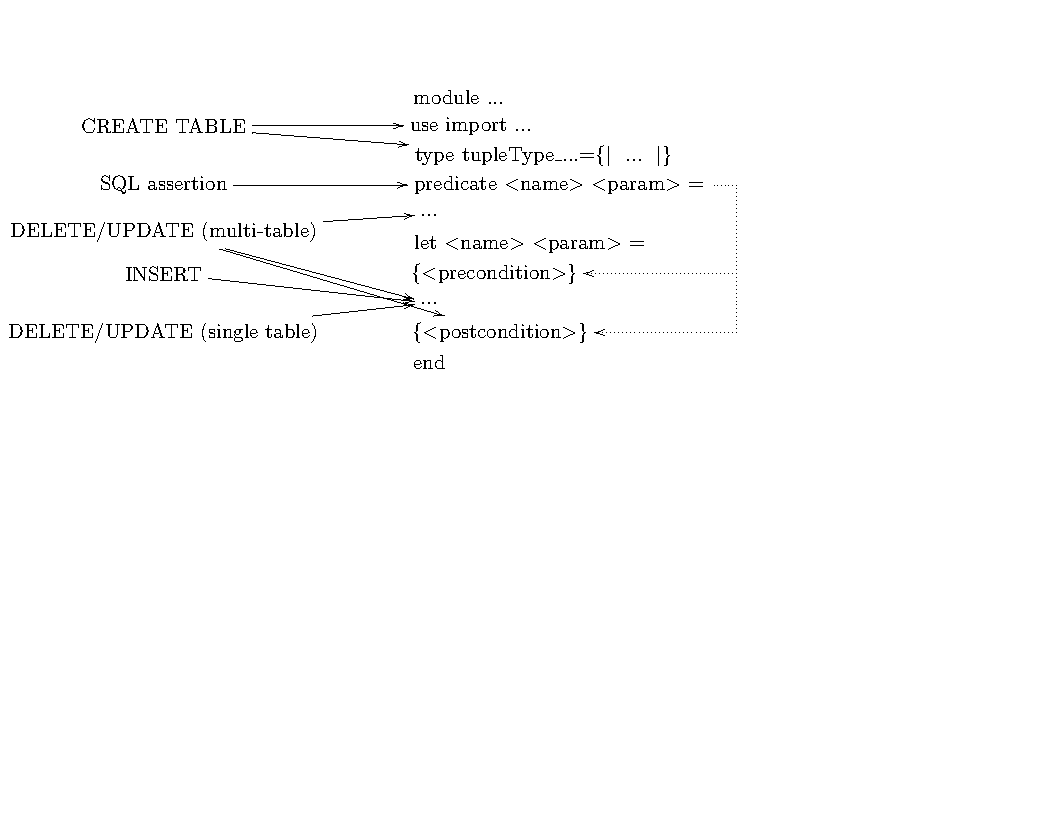
\includegraphics[scale=0.9]{structure.pdf}
\end{frame}

\section[8.\ Problem and Solution --\!\!]{Problem and Solution}
\begin{frame}[fragile]
\frametitle{Problem and Solution}
\only<1>
{
Our former experiments show that our methods cannot detect some safe date modification operators when the integrity constraint $C$ is in the form of:
% \begin{equation}
\[
  \exists x \in R, f(x)
\label{existsequ}
\]
% \end{equation}

Before $U$ is executed:
\[
r \models C(r) \equiv \exists x \in r, f(x)
\]

What we want to proof:
\[
\Ur \models C(\Ur) \equiv \exists x \in \Ur, f(x)
\]

}

\only<2>
{
We adopt the predicate transformer to improve it:

e.g. backward predicate transformer $\lvec{U}$
\[
\mathcal{B} \models \lvec{U} (C) \Rightarrow \UB \models C  
\]

Use this method, our problem becomes: $C \Rightarrow \lvec{U} (C)$

}

\only<3>
{
For the constraints in the following form:
\[
% \begin{equation}
  \exists x \in R, f(x)
\label{existsequ}
% \end{equation}
\]

We find precise predicate transformer $C'$:
\[
\mathcal{B} \models C' \Leftrightarrow \UB \models C
\]

}

\only<4>
{

\begin{theorem}
The execution of any SQL INSERT statements will not affect the constraint $C$.
\end{theorem}


\begin{theorem}
$
\Ur \models C \Leftrightarrow \exists x \in r, f(x) \land \lnot g(x)
$
\end{theorem}


\begin{theorem}
$
  \Ur \models C \Leftrightarrow \exists x \in r, ( f(x) \land \lnot g(x) ) \lor ( g(x) \land f(\sigma(x)) )
$
\end{theorem}

}

\only<5>
{
Similar results can be derived when the constraint $C$ is in the form of:
% \begin{equation}
\[
\forall x \in R, f(x)
\label{forallequ}
\]
% \end{equation}

Before $U$ is executed:
\[
r \models C(r) \equiv \forall x \in r, f(x)
\]

What we want to proof:
\[
\Ur \models C(\Ur) \equiv \forall x \in \Ur, f(x)
\]
}

\only<6>
{
\begin{theorem}
$
\Ur \models C \Leftrightarrow f(t)
$
\end{theorem}

\begin{theorem}
The execution of any SQL DELETE statements will not affect the constraint $C$.
\end{theorem}

\begin{theorem}
$
\Ur \models C \Leftrightarrow \forall x \in r, \lnot g(x) \lor ( g(x) \land f(\sigma(x)) )
$
\end{theorem}
}

\end{frame}


\section[9.\ Experiments --\!\!]{Experiments}
\begin{frame}[fragile]
\frametitle{Experiments}

\only<1>
{
% Provers: Alt-Ergo, CVC3, Yices and Gappa.
\begin{block}{Provers}
Alt-Ergo, CVC3, Yices and Gappa.
\end{block}

Unsafe data modification operations can be detected correctly.

For safe data modification operations:
\begin{center}
\begin{tabular}{|c|c|c|c|}
\hline
& INSERT & DELETE & UPDATE \\
\hline
least mean time (s) & 0.205 & 2.338 & 1.149 \\
\hline
\end{tabular}
\end{center}
}

\only<2>
{
When the integrity constraint $C$ is in the form of:
\[
  \exists x \in R, f(x)
\label{existsequ}
\]

We try a newer version of Why3 (0.72) and find that the weakest precondition approach can detect safe data modification operations.

\begin{tabular}{|c|c|c|c|}
\hline
& INSERT & DELETE & UPDATE \\
\hline
% 最弱前置条件 & & & \\
weakest precondition (s) & 0.208 & 0.119 & 0.381 \\
\hline
% 等价验证条件 & & & \\
% equivalent condition
precise predicate transformer (s) & 0 & 0.047 & 0.054 \\
\hline
\end{tabular}
}

\only<3>
{
When the integrity constraint $C$ is in the form of:
\[
\forall x \in R, f(x)
\label{forallequ}
\]


\begin{tabular}{|c|c|c|c|}
\hline
& INSERT & DELETE & UPDATE \\
\hline
% 最弱前置条件 & & & \\
weakest precondition (s) & 0.199 & 0.16 & 0.323 \\
\hline
% 等价验证条件 & & & \\
% equivalent condition
precise predicate transformer (s)& 0.056 & 0 & 0.055 \\
\hline
\end{tabular}
}

\end{frame}

% \section[5.\ SQL update functions --\!\!]{SQL update functions}
% 
% \begin{frame}[fragile]
% % \frame{
% \frametitle{SQL update functions}
% 
% \only<1>{
% For example, we have the following two tables:
% \begin{alltt}
% CREATE TABLE r
% (a1: INTEGER, a2: INTEGER);
% \end{alltt}
% 
% \begin{alltt}
% CREATE TABLE r1
% (b1: INTEGER, b2: INTEGER);
% \end{alltt}
% % \bdm
% % \begin{array}{l}
% %   \mbox{CREATE TABLE r} \\
% %   \mbox{(a1: INTEGER, a2: INTEGER);}
% % \end{array}
% % &&
% % \begin{array}{l}
% %   \mbox{CREATE TABLE r1} \\
% %   \mbox{(b1: INTEGER, b2: INTEGER);}
% % \end{array}
% % \edm
% }
% 
% \begin{itemize}
%   \item<2> {\color{blue}{SQL insert}}
%   \only<2>{
%   Insert a tuple into table r.
%   % \begin{itemize}
%   % \begin{center}
% %  \item explicit way:
% %	\begin{alltt}
% %	INSERT INTO r (a1,a2)
% % 	VALUES (1,1);
% %	\end{alltt}
%   %\item implicit way:
% 	\begin{alltt}
%  	INSERT INTO r
%  	VALUES (1,1);
% 	\end{alltt}
% % 	\begin{altt}
% % 	INSERT INTO r (a1,a2) \\
% % 	VALUES (1,1); \\
% % 	INSERT INTO r1 \\
% % 	VALUES (1,1);
% % 	\end{altt}
%   % \end{center}
%   %\end{itemize}
%   }
% \item<3> {\color{blue}{SQL delete}}
%   \only<3>{
%   Delete tuples which satisfy the condition in the WHERE clause.
%   \begin{itemize}
%   % \begin{center}
%   \item only contains a single table:
% 	\begin{alltt}
% 	DELETE FROM r \\
% 	WHERE ( r.a1 = 1 );
% 	\end{alltt}
%   \item contains multiple tables:
% 	\begin{alltt}
% 	DELETE FROM r \\
% 	USING r, r1 \\
% 	WHERE ( r.a1 = r1.b1 );
% 	\end{alltt}
%   % \end{center}
%   \end{itemize}
%   }
% \item<4> {\color{blue}{SQL update}}
%   \only<4>{
%   Update tuples which satisfy the condition in the WHERE clause.
%   \begin{itemize}
%   % \begin{center}
%   \item only contains a single table:
% 	\begin{alltt}
% 	UPDATE r \\
% 	SET r.a1 = 1, r.a2 = 2 \\
% 	WHERE ( r.a1 = r.a2 );
% 	\end{alltt}
%   \item contains multiple tables:
% 	\begin{alltt}
% 	UPDATE r \\
% 	SET r.a1 = 1 \\
% 	FROM r, r1 \\
% 	WHERE ( r.a1 = r1.b1 );
% 	\end{alltt}
%   % \end{center}
%   \end{itemize}
% %   \begin{center}
% % 	UPDATE r \\
% % 	SET r.a1 = 1, r.a2 = 2 \\
% % 	WHERE ( r.a1 = r.a2 ); \\
% % 	UPDATE r \\
% % 	SET r.a1 = 1 \\
% % 	FROM r, r1 \\
% % 	WHERE ( r.a1 = r1.b1 );
% %   \end{center}
%   }
% \end{itemize}
% % }
% \end{frame}
% 
% \section[3.\ SQL assertion --\!\!]{SQL assertion}
% 
% \begin{frame}[fragile]
% % \frame{
% \frametitle{SQL assertion}
% 
% % \begin{right}
% %   \mbox{CREATE ASSERTION $<$assertion name$>$} \\
% %   \mbox{CHECK $<$search condition$>$}
% % \end{right}
% % $<$search condition$>$ can be translated into a logical formula:
% 
% An assertion can be viewed as a formula that specifies the valid state of a database.
% 
% For example,
% \begin{verbatim}
% CREATE ASSERTION assertion1
% CHECK (NOT EXISTS (SELECT *
%                    FROM r x
%                    WHERE x.a1 <> x.a2));
% \end{verbatim}
% % \begin{flushright}
% % \mbox{CREATE ASSERTION assertion1} \\
% % \mbox{CHECK (NOT EXISTS (SELECT *} \\
% % \mbox{FROM r x} \\
% % \mbox{WHERE x.a1 $<>$ x.a2));} \\
% % \end{flushright}
% can be viewed as:
% \bdm
% \mbox{assertion1: } \lnot ( \exists x \in r;~ x.a1 \neq x.a2 )
% \edm
% % }
% \end{frame}
% 
% \section[4.\ Proposed solution --\!\!]{Proposed solution}
% 
% \begin{frame}[fragile]
% % \frame{
% \frametitle{Proposed solution}
% % We use weakest precondition $wpc$ to prove the target.
% 
% Given a constraint $C$ and a SQL update $f$,
% firstly we use Why3 to generate the weakest precondition $wpc(f,C)$.
% \\
% Next we call the provers to prove $C \Rightarrow wpc(f,C)$, if it is proven, then $f(B) \models C$.
% 
% % \only<1>{
% % \begin{displaymath}
% % f, C \longrightarrow wpc(f, C) \longrightarrow (C \Rightarrow wpc(f,C)) \longrightarrow f(B) \models C
% % \end{displaymath}
% % }
% % \only<2>{
% % \begin{center}
% % Find $\phi$, s.t. $f(B) \models \phi$:
% % \end{center}
% % \begin{displaymath}
% % f, C, \phi \longrightarrow wpc(f, C \land \phi) \longrightarrow (C \Rightarrow wpc(f,C \land \phi))
% % \end{displaymath}
% % \begin{displaymath}
% % \longrightarrow f(B) \models (C \land \phi) \longrightarrow f(B) \models C
% % \end{displaymath}
% % }
% % \only<3>{
% Our major work is:
% \begin{itemize}
%   \item Translate SQL assertion into predicate in Why3
%   \item Translate SQL INSERT, DELETE, UPDATE into functions in Why3
% \end{itemize}
% % }
% % }
% \end{frame}
% 
% \section[5.\ Translation Overiew --\!\!]{Translation Overiew}
% \begin{frame}[fragile]
% \frametitle{Translation Overiew}
%  \begin{center}
% %   \includegraphics[scale=0.8]{pic3.pdf}
%  \end{center}
% % \scalebox{1} % Change this value to rescale the drawing.
% % {
% % \begin{pspicture}(0,-3.4575)(11.85375,3.4575)
% % \usefont{T1}{ptm}{m}{n}
% % \rput(2.2929688,2.5325){CREATE TABLE}
% % \usefont{T1}{ptm}{m}{n}
% % \rput(2.5365624,1.3925){assertion}
% % \usefont{T1}{ptm}{m}{n}
% % \rput(2.393125,0.4125){DELETE/UPDATE(multi-tables)}
% % \usefont{T1}{ptm}{m}{n}
% % \rput(2.7346876,-1.7275){INSERT}
% % \usefont{T1}{ptm}{m}{n}
% % \rput(2.413125,-2.5475){DELETE/UPDATE(single table)}
% % \usefont{T1}{ptm}{m}{n}
% % \rput(8.024375,3.2725){module ...}
% % \usefont{T1}{ptm}{m}{n}
% % \rput(8.255781,2.7125){use import ...}
% % \usefont{T1}{ptm}{m}{n}
% % \rput(8.486563,1.8925){type ... = {| ... |}}
% % \usefont{T1}{ptm}{m}{n}
% % \rput(9.5525,1.0125){predicate  <name>  <param> =}
% % \usefont{T1}{ptm}{m}{n}
% % \rput(7.433125,0.3925){...}
% % \usefont{T1}{ptm}{m}{n}
% % \rput(8.966562,-0.3675){let <name> <param> =}
% % \usefont{T1}{ptm}{m}{n}
% % \rput(8.633437,-1.1275){{ <precondition> }}
% % \usefont{T1}{ptm}{m}{n}
% % \rput(7.433125,-1.8475){...}
% % \usefont{T1}{ptm}{m}{n}
% % \rput(8.703438,-2.6275){{ <postcondition> }}
% % \usefont{T1}{ptm}{m}{n}
% % \rput(7.5675,-3.3075){end}
% % \psline[linewidth=0.04cm,arrowsize=0.05291667cm 2.0,arrowlength=1.4,arrowinset=0.4]{->}(3.83375,2.6275)(7.23375,2.6475)
% % \psline[linewidth=0.04cm,arrowsize=0.05291667cm 2.0,arrowlength=1.4,arrowinset=0.4]{->}(3.87375,2.4875)(7.21375,1.9275)
% % \psline[linewidth=0.04cm,arrowsize=0.05291667cm 2.0,arrowlength=1.4,arrowinset=0.4]{->}(3.77375,1.5675)(7.19375,1.0275)
% % \psline[linewidth=0.04cm,arrowsize=0.05291667cm 2.0,arrowlength=1.4,arrowinset=0.4]{->}(4.95375,0.4875)(7.25375,0.7475)
% % \psline[linewidth=0.04cm,arrowsize=0.05291667cm 2.0,arrowlength=1.4,arrowinset=0.4]{->}(4.79375,0.1875)(7.21375,-1.6725)
% % \psline[linewidth=0.04cm,arrowsize=0.05291667cm 2.0,arrowlength=1.4,arrowinset=0.4]{->}(3.57375,-1.7125)(7.15375,-1.7525)
% % \psline[linewidth=0.04cm,arrowsize=0.05291667cm 2.0,arrowlength=1.4,arrowinset=0.4]{->}(4.85375,-2.4925)(7.19375,-1.9125)
% % \psline[linewidth=0.04cm,arrowsize=0.05291667cm 2.0,arrowlength=1.4,arrowinset=0.4]{->}(4.55375,0.1075)(7.27375,-2.6725)
% % \psline[linewidth=0.04,arrowsize=0.05291667cm 2.0,arrowlength=1.4,arrowinset=0.4]{->}(11.81808,0.8275)(11.83375,-2.5525)(10.31375,-2.5525)
% % \psline[linewidth=0.04,arrowsize=0.05291667cm 2.0,arrowlength=1.4,arrowinset=0.4]{->}(11.519584,0.8275)(11.53375,-1.1725)(10.17375,-1.1532692)
% % \end{pspicture}
% % }
% \end{frame}
% 
% 
% \section[6.\ Demo --\!\!]{Demo}
% 
% \begin{frame}
%   \frametitle{Demo}
%   \begin{center}
%   Demo
% \end{center}
% \end{frame}
% % \begin{frame}[fragile]
% % \frametitle{Example}
% % A simple example:
% %
% % SQL assertion is defined as:
% % % \begin{center}
% % % \begin{lstlisting}
% % \begin{verbatim}
% % CREATE ASSERTION myassertion
% % CHECK (EXISTS (SELECT *
% % 	       FROM r x
% % 	       WHERE x.a1 IN (1, 2, 3) ));
% % \end{verbatim}
% % % \end{lstlisting}
% % SQL update function:
% % \begin{center}
% % % \begin{lstlisting}
% % \begin{verbatim}
% % INSERT INTO r
% % VALUES (1,1);
% % \end{verbatim}
% % % \end{lstlisting}
% % \end{center}
% % \end{frame}
% %
% % \begin{frame}[fragile]
% % The target Why3ML code:
% % \begin{verbatim}
% % module Test
% % use import int.Int
% % use import list.Append
% % use import list.List
% % use import list.Mem
% % type tupleType_r = {| a1: int; a2: int |}
% % predicate myassertion ( r: list tupleType_r )  =
% %  ( exists x: tupleType_r. mem x r
% % /\  mem x.a1 (  (Cons 1 (Cons 2 (Cons 3 Nil) ) )  )  )
% % let insert  ( r: list tupleType_r )  =
% % { myassertion r }
% % r ++ ( Cons {| a1 = 1; a2 = 1 |} Nil)
% % { myassertion result }
% % end
% % \end{verbatim}
% % \end{frame}
% 
% \begin{frame}[fragile]
% \frametitle{Demo}
% A more complex example:
% 
% SQL assertion is defined as:
% \begin{center}
% % \begin{lstlisting}
% \begin{verbatim}
% CREATE ASSERTION example
% CHECK (NOT EXISTS (SELECT *
% 	       FROM r x,r1 x1
% 	       WHERE x.a1 <> x1.b1) );
% \end{verbatim}
% \end{center}
% % \end{lstlisting}
% SQL DELETE with multi-tables involved.
% \begin{center}
% % \begin{lstlisting}
% \begin{verbatim}
% DELETE FROM r
% USING r, r1
% WHERE ( r.a1 = r1.b1 );
% \end{verbatim}
% % \end{lstlisting}
% \end{center}
% \end{frame}
% 
% \begin{frame}[fragile]
% The semantics of this function is (pseudo-code):
% % \include{eg1-1}
% % \begin{lstlisting}[language=Ocaml]
% % \begin{lstlisting}[language=C]
% \begin{verbatim}
% foreach tuple y in r1
% do
%         get y.b1;
%         foreach tuple x in r
%         do
%                 get x.a1;
%                 if x.a1 = y.b1 then
%                         delete x from r
%         done
% done
% \end{verbatim}
% % \end{lstlisting}
% \end{frame}
% 
% \begin{frame}[fragile]
% We rewrite it as (pseudo-code):
% % \begin{lstlisting}[language=C]
% \begin{verbatim}
% foreach tuple x in r
% do
%         get x.a1;
%         foreach tuple y in r1
%         do
%                 flag := False;
%                 get y.b1;
%                 if x.a1 = y.b1 then
%                         flag := True
%         done;
%         if flag = True then
%                 delete x from r
%   done
% \end{verbatim}
% % \end{lstlisting}
% \end{frame}
% 
% % \begin{frame}[fragile]
% % Translate it into Why3ML code:
% % % \begin{lstlisting}
% % {\tiny
% % \begin{verbatim}
% % type tupleType_r = {| a1: int; a2: int |}
% % type tupleType_r1 = {| b1: int; b2: int |}
% % predicate example ( r: list tupleType_r )  ( r1: list tupleType_r1 )  =
% %  ( not ( exists x1: tupleType_r1, x: tupleType_r. mem x1 r1 /\  mem x r /\ x.a1 <> x1.b1 )  )
% % predicate sc_predicate ( r1_b1_value: int ) ( r_a1_value: int ) =
% %  ( r_a1_value = r1_b1_value )
% % let rec iter_r1 r_a1_value r1 =
% % { true }
% % match r1 with
% % | Nil -> False
% % | Cons {| b1 = r1_b1_value; b2 = r1_b2_value |} l ->
% % 	if  ( r_a1_value = r1_b1_value )  then True
% % 	else ( iter_r1 r_a1_value l )
% % end
% % { true /\ ( result = True <->
% % exists x_r1: tupleType_r1. mem x_r1 r1 /\ ( sc_predicate x_r1.b1 r_a1_value ) ) }
% % let rec delete_r r1 r =
% % { true }
% % match r with
% % | Nil -> Nil
% % | Cons {| a1 = r_a1_value; a2 = r_a2_value |} l ->
% % 	if ( iter_r1 r_a1_value r1 ) then ( delete_r r1 l )
% % 	else Cons {| a1 = r_a1_value; a2 = r_a2_value |} ( delete_r r1 l )
% % end
% % { example r r1 -> example r r1 /\
% % forall x_r: tupleType_r.  mem x_r r ->
% % not ( exists x_r1: tupleType_r1. mem x_r1 r1 /\ ( sc_predicate x_r1.b1 x_r.a1 ) )  }
% % \end{verbatim}
% % }
% % % \end{lstlisting}
% % \end{frame}
% 
% 
% 
% % \only<2>{
% % The semantics of this function is:
% % % \begin{lstlisting}[language=C]
% % \begin{lstlisting}
% %   foreach tuple y in r1
% %   do
% %     get y.b1;
% %   	foreach tuple x in r
% % 	do
% % 		get x.a1;
% % 		if x.a1 = y.b1 then
% % 			delete x from r
% % 	done
% %   done
% % \end{lstlisting}
% % }
% %
% % \only<3>{
% % We rewrite it as:
% % \begin{lstlisting}[language=C]
% %   foreach tuple x in r
% %   do
% %     get x.a1;
% % 	foreach tuple y in r1
% % 	do
% % 		get y.b1;
% % 		if x.a1 = y.b1 then
% % 			flag = True
% % 		else
% % 			flag = False;
% % 	done;
% % 	if flag = True then
% % 		delete x from r
% %   done
% % \end{lstlisting}
% % }
% %
% % \only<4>{
% % Translate it into Why3ML code:
% % \begin{lstlisting}[language=Ocaml]
% % type tupleType_r = {| a1: int; a2: int |}
% % type tupleType_r1 = {| b1: int; b2: int |}
% % predicate example ( r: list tupleType_r )  ( r1: list tupleType_r1 )  =
% %  ( not ( exists x1: tupleType_r1, x: tupleType_r. mem x1 r1 /\  mem x r /\ x.a1 <> x1.b1 )  )
% % predicate sc_predicate ( r1_b1_value: int ) ( r_a1_value: int ) =
% %  ( r_a1_value = r1_b1_value )
% % let rec iter_r1 r_a1_value r1 =
% % { true }
% % match r1 with
% % | Nil -> False
% % | Cons {| b1 = r1_b1_value; b2 = r1_b2_value |} l ->
% % 	if  ( r_a1_value = r1_b1_value )  then True
% % 	else ( iter_r1 r_a1_value l )
% % end
% % { true /\ ( result = True <->
% % exists x_r1: tupleType_r1. mem x_r1 r1 /\ ( sc_predicate x_r1.b1 r_a1_value ) ) }
% % let rec delete_r r1 r =
% % { true }
% % match r with
% % | Nil -> Nil
% % | Cons {| a1 = r_a1_value; a2 = r_a2_value |} l ->
% % 	if ( iter_r1 r_a1_value r1 ) then ( delete_r r1 l )
% % 	else Cons {| a1 = r_a1_value; a2 = r_a2_value |} ( delete_r r1 l )
% % end
% % { example r r1 -> example r r1 /\
% % forall x_r: tupleType_r. mem x_r r ->
% % exists x_r1: tupleType_r1. mem x_r1 r1 /\ ( sc_predicate x_r1.b1 x_r.a1 ) }
% % \end{lstlisting}
% % }
% % \end{frame}
% 


\section[10.\ Conclusion \& Prospect --\!\!]{Conclusion \& Prospect}
\begin{frame}
\frametitle{Conclusion \& Prospect}

\only<1>
{
Our work:
\begin{itemize}
  \item rules of reducing SQL database integrity constraints to assertions.
  \item translating SQL assertions into first-order logical formulae.
  \item semantics of SQL data modification operations (INSERT/DELETE/UPDATE).
  \item using weakest precondition and Why3 to implement automated verification of database integrity constraints.
\end{itemize}
}

\only<2>
{
Future work:
\begin{itemize}
  \item more complex SQL grammar.
  \item aggregate functions.
\end{itemize}
}
%   \begin{itemize}
% 	\item Automated proof of some database assertions.
% 	\item Future work:
% 	  \begin{itemize}
% 		  % 
% 		\item complete SQL grammar?
% 		\item aggregate functions 
% 	  \end{itemize}
% 	\end{itemize}
\end{frame}
\end{document}
